\section{Experiments}
\label{section:experiments}


As Headless-AD extends and improves on AD, we checked it in two different aspects. Firstly, it should maintain In-Context Learning abilities and thus generalize well to new tasks. Secondly, it should show high performance on action spaces different from the one seen during training. All of the following environments are designed specifically to check both of the above aspects. In our experiments, we used the TinyLLaMa \citep{zhang2024tinyllama} implementation of the transformer model and AdamW optimizer \citep{loshchilov2017decoupled}. All environment specific hyperparameters are listed in \Cref{appendix:hypers}.

\subsection{Bernoulli Bandit}
\label{eval:bernoulli_bandit}


\begin{figure*}[t]
    \vskip 0.2in
    \centering
    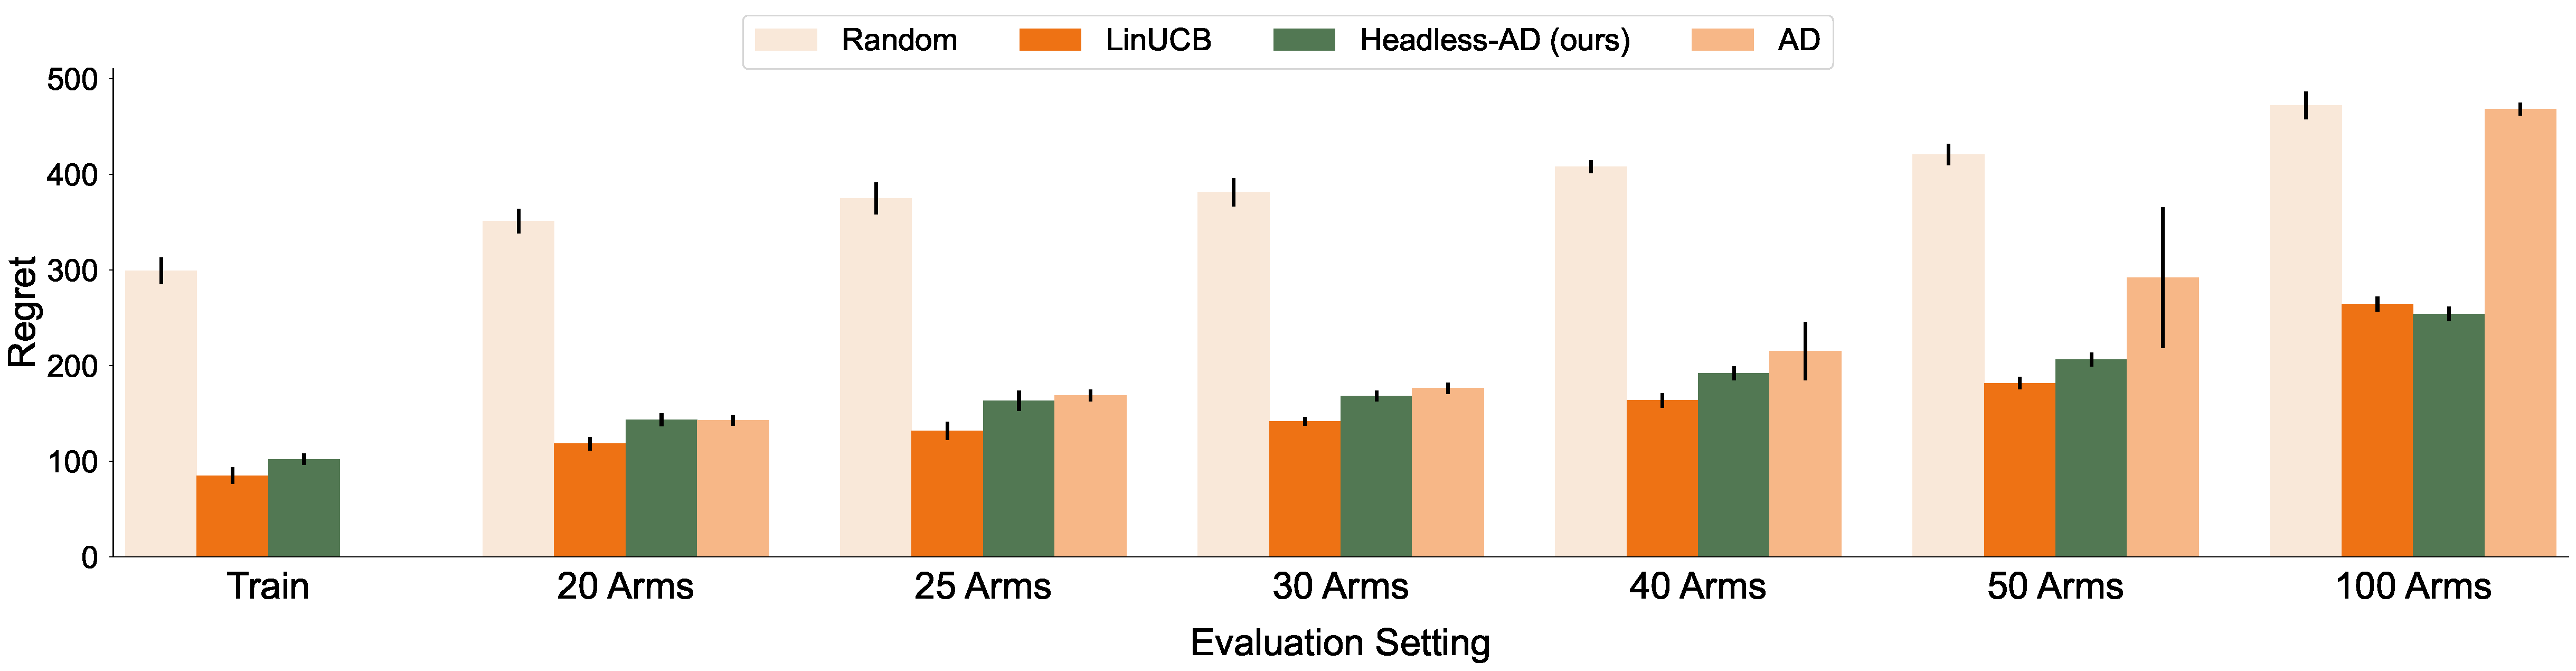
\includegraphics[width=\textwidth]{images/contextual_bars.pdf}
    \caption{\textbf{Contextual Bandit Regret Comparison:} The \textit{Train} set consists of trajectories of LinUCB trained for $300$ steps on contextual bandits with $4-20$ arms. All models are also evaluated for $300$ steps. The results are averaged over $5$ seeds, each seed containing $100$ environments. AD requires retraining on each new action set and, while showing good performance on lower space sizes, it fails to converge on larger ones. Due to its variable-size action sets, AD was not tested on the \textit{Train} set. Conversely, Headless-AD, trained exclusively on the \textit{Train} set, is successful at both learning effectively within this environment and generalizing to new action sets. }
    \label{fig:contextual}
    \vskip -0.2in
\end{figure*}

\textbf{Motivation:}
This experiment checked Headless-AD's abilities on a toy task, where the environment did not have a notion of state and returned binary rewards.

\textbf{Setup 1:} In our first experiment, we examined the model's robustness to distributional shifts in rewards. We used a Bernoulli bandit where each arm is associated with a mean $\mu$ and the reward after pulling an arm $i$ is generated by $\text{Bernoulli}(\mu)$. The training dataset consisted of bandits with $4-20$ arms, i.e., different action set sizes. Additionally, to evaluate the ICL capabilities of models, the reward distribution over the arms differed between train and test \citep{laskin2022context}. Specifically, the training data consisted of bandits where in $95\%$ of cases the odd-numbered arms were assigned a random $\mu \in [0.5, 1]$ and even-numbered arms received $\mu \in [0, 0.5]$. For other $5\%$ of bandits, the ranges were swapped between odd and even arms. The test distribution also consisted of bandits with $4-20$ arms, but the reward distribution was switched either to even arms or was uniform, i.e., all arms were assigned $\mu \in [0, 1]$. Learning histories were generated using Thompson Sampling algorithm for a total of $10,000$ bandit instances with $300$ steps each. The evaluation was performed on $100$ bandits in each reward distribution, included $5$ seeds, and the algorithms were rolled out for $300$ steps.

\textbf{Results and Discussion 1:} As depicted in \Cref{fig:bandit_new_regrets}, the Headless-AD model demonstrates strong generalization capabilities by almost reaching the performance results set by the traditional Thompson Sampling algorithm under each test distribution. 

\textbf{Setup 2:} In our second experiment, we evaluated the transferability of Headless-AD to new action set sizes. Training distribution remained the same as in the previous experiment. Each evaluation dataset consisted of a fixed amount of $20$, $25$, $30$, $40$ and $50$ arms and a uniform distribution of rewards. AD was trained on fixed-size bandits corresponding to each evaluation dataset. The training and evaluation reward distributions were the same as for Headless-AD.

\textbf{Results and Discussion 2:} \Cref{fig:bandit_together_curves} shows that Headless-AD can effectively maintain its performance as the action space grows, without necessitating any retraining. Moreover, Headless-AD even outperforms a specially trained AD, especially on larger action sets. Note that Headless-AD's performance curves resemble TS's performance curves, signifying that it has indeed learned a policy improvement operator generic enough to apply to unseen action set sizes.

\subsection{Contextual Bandit}
\label{eval:contextual_bandit}

\textbf{Motivation:} To validate the sustained performance of Headless-AD, we progressed to a more complex Multi-Armed Bandit (MAB) extension that integrated states and real-valued rewards.

\textbf{Setup:} Each time step presented a context with arm features modeled as two-dimensional vectors, and rewards were generated with a standard deviation $\sigma = 1$. The data were created using a LinUCB \cite{li2010contextual} algorithm trained over $300$ steps, on bandits with $4-20$ arms. We used $100$ contextual bandits, $5$ seeds and $300$ evaluation steps.

\textbf{Results and Discussion:} As shown in \Cref{fig:contextual}, Headless-AD's performance is on par with LinUCB across varied arm counts. While AD also reaches the performance of LinUCB on lower space sizes, it has problems converging on larger action space sizes, in addition to requiring a specific retraining. This serves to highlight the advantages of Headless-AD for use in even more complex environments than toy Bernoulli bandits.


\begin{figure*}[t]
    \vskip 0.2in
    \centering
    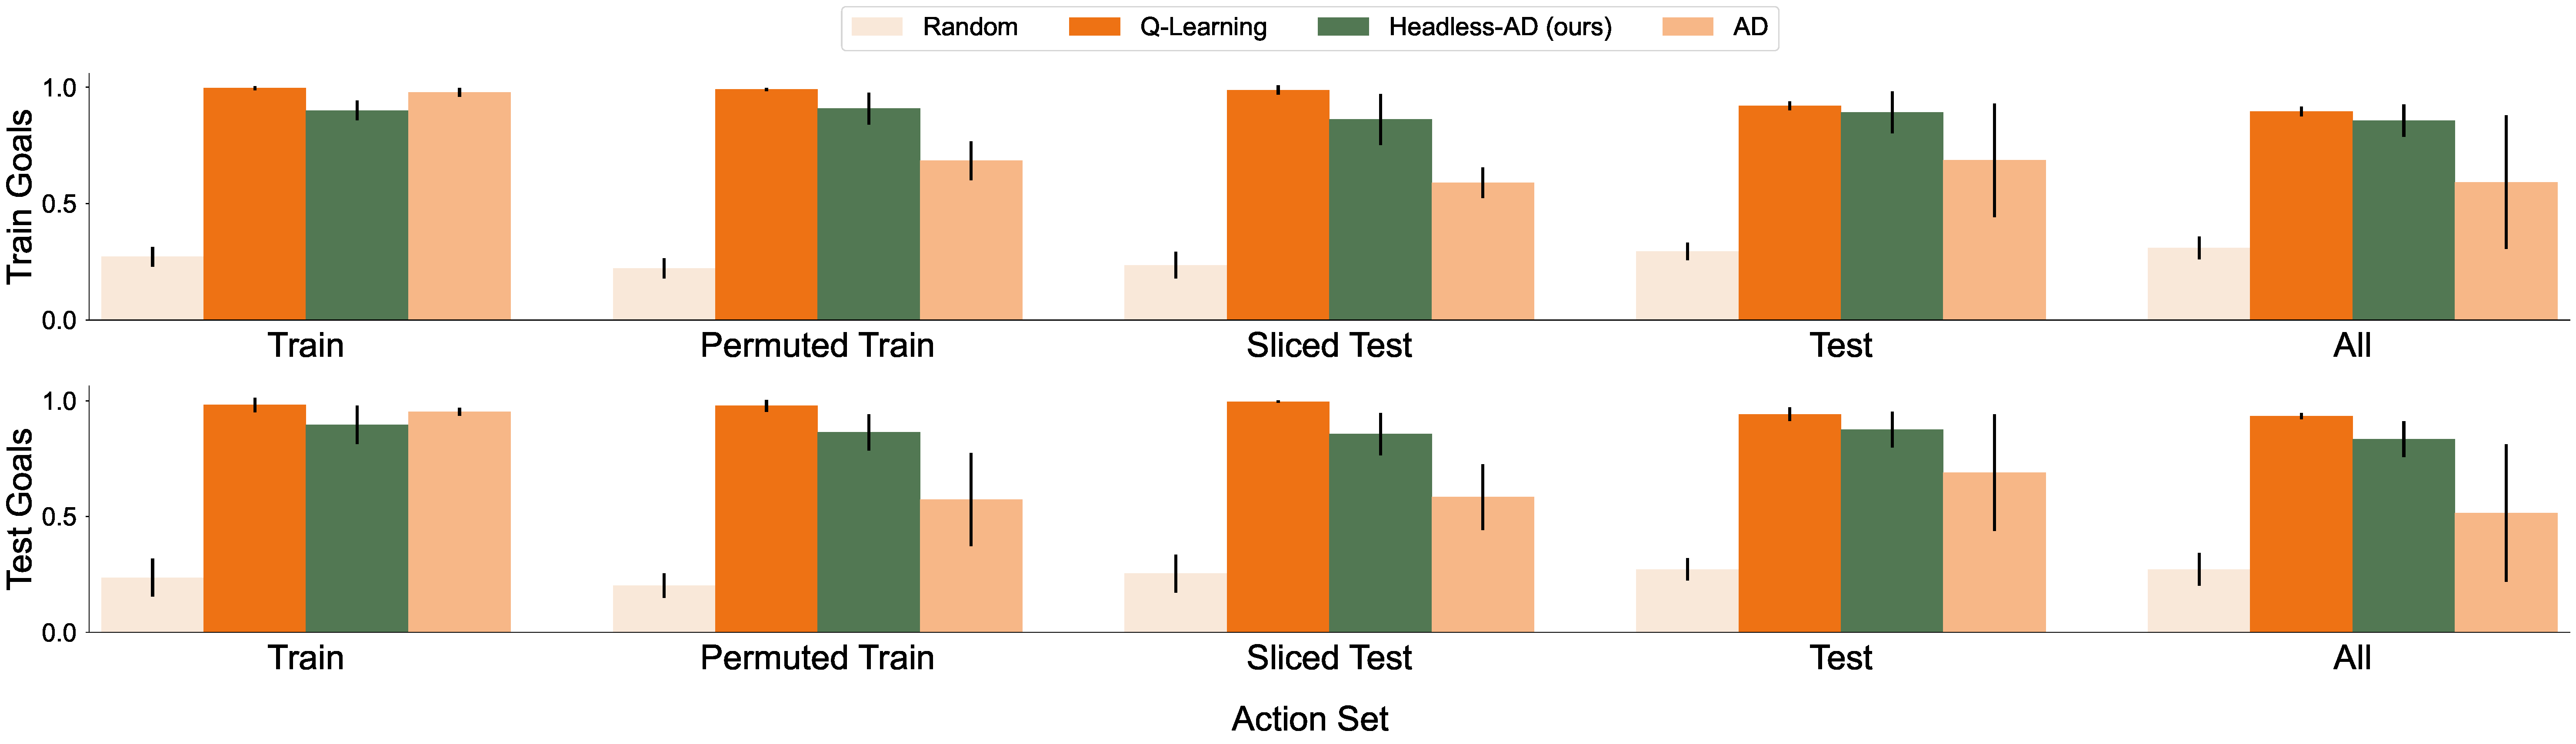
\includegraphics[width=0.95\textwidth]{images/gridworld_bars.pdf}
    \caption{\textbf{Darkroom Environment Success Rate:} The chart displays mean success rates and their standard deviations from five training seeds, comparing performance in fixed and variable action spaces, along with the models' adaptability to new goals. \textit{Train Actions} refers to the fixed-size action set used for training. \textit{Test Actions} include exclusively unseen actions, while \textit{All Actions} combine both \textit{Train} and \textit{Test}, with set sizes expanded to $75$ and $125$ respectively. Since the output dimension changes, AD requires retraining. To assess AD's adaptability to the changed action semantics, we either permute \textit{Train Actions} or replace it with the first $50$ actions from the \textit{Test} set. In this case, AD does not require retraining, but it still exhibits diminished performance. Conversely, Headless-AD, while trained solely on \textit{Train Actions}, delivers strong and stable performance across all action set variants, and even surpasses specially trained AD on larger set sizes.}
    \label{fig:gridworld_bars}
    \vskip -0.2in
\end{figure*}

\subsection{Darkroom}
\label{sec:exp_gridworld}

\textbf{Motivation:} In this experiment, we delve into a more sophisticated Markov Decision Process (MDP) framework, constructing five distinct action spaces aimed at demonstrating the architectural constraints of AD. We then show how Headless-AD's architecture is engineered to navigate the complexities presented by each of these diverse action sets.

\textbf{Setup:} The Darkroom environment, inspired by \citet{chevalier2018minimalistic} and \citet{jain2020generalization}, consists of a $N \times N$ grid where the agent needs to reach a specific cell for a reward. In our experiment, the action space consisted of $3$-step sequences of $5$ atomic actions: \textit{up}, \textit{down}, \textit{left}, \textit{right}, \textit{noop}. As a result, the environment offered $5^3$ possible actions. The agent earned a reward of $1$ if the trajectory induced by the action sequence passed through a goal cell, after which the episode finished. Otherwise, the reward was $0$. As an observation, the environment offered only the current coordinates of the agent, so the goal information could only be obtained from the agent's memory. We divided the goals into disjoint sets used for training and testing in order to evaluate Headless-AD's in-context learning abilities. Furthermore, the action set was randomly split into train and test sets, each including $50$ and $75$ actions respectively, to create five distinct spaces for assessing various generalization aspects. These action sets are visualized in \Cref{fig:action_sets_viz}.

\textbf{Train Actions.} Comprising the training split, this set represented the actions encountered during model training.

\textbf{Test Actions.} Comprising the test split, this set assessed Headless-AD's generalization on novel and larger action sets.

\textbf{All Actions.} Combining both training and testing actions, this set contained $125$ actions and was $2.5$ times larger than the training set. Its aim was to challenge Headless-AD to effectively integrate seen and unseen actions.

\textbf{Permuted Train Actions.} Shuffled training set, meant to test the model's adaptability to reordered action spaces that comprised of the same actions.

\textbf{Sliced Test Actions.} Tailored to match the training set size, this set contained a slice of the first $50$ actions from the test set. Its aim was to check the models' generalization abilities on unseen actions while maintaining the action set size.

In scenarios where the action space exceeded the size of the training set, we analyzed the performance of an AD model retrained from scratch. The data generation algorithm was Q-learning, executed over $200$ episodes for each environment. Further details on model hyperparameters are available in \Cref{appendix:hypers}.


% \begin{figure*}[t]
%     \vskip 0.2in
%     \centering
%     \begin{subfigure}{\columnwidth}
%         \centering
%         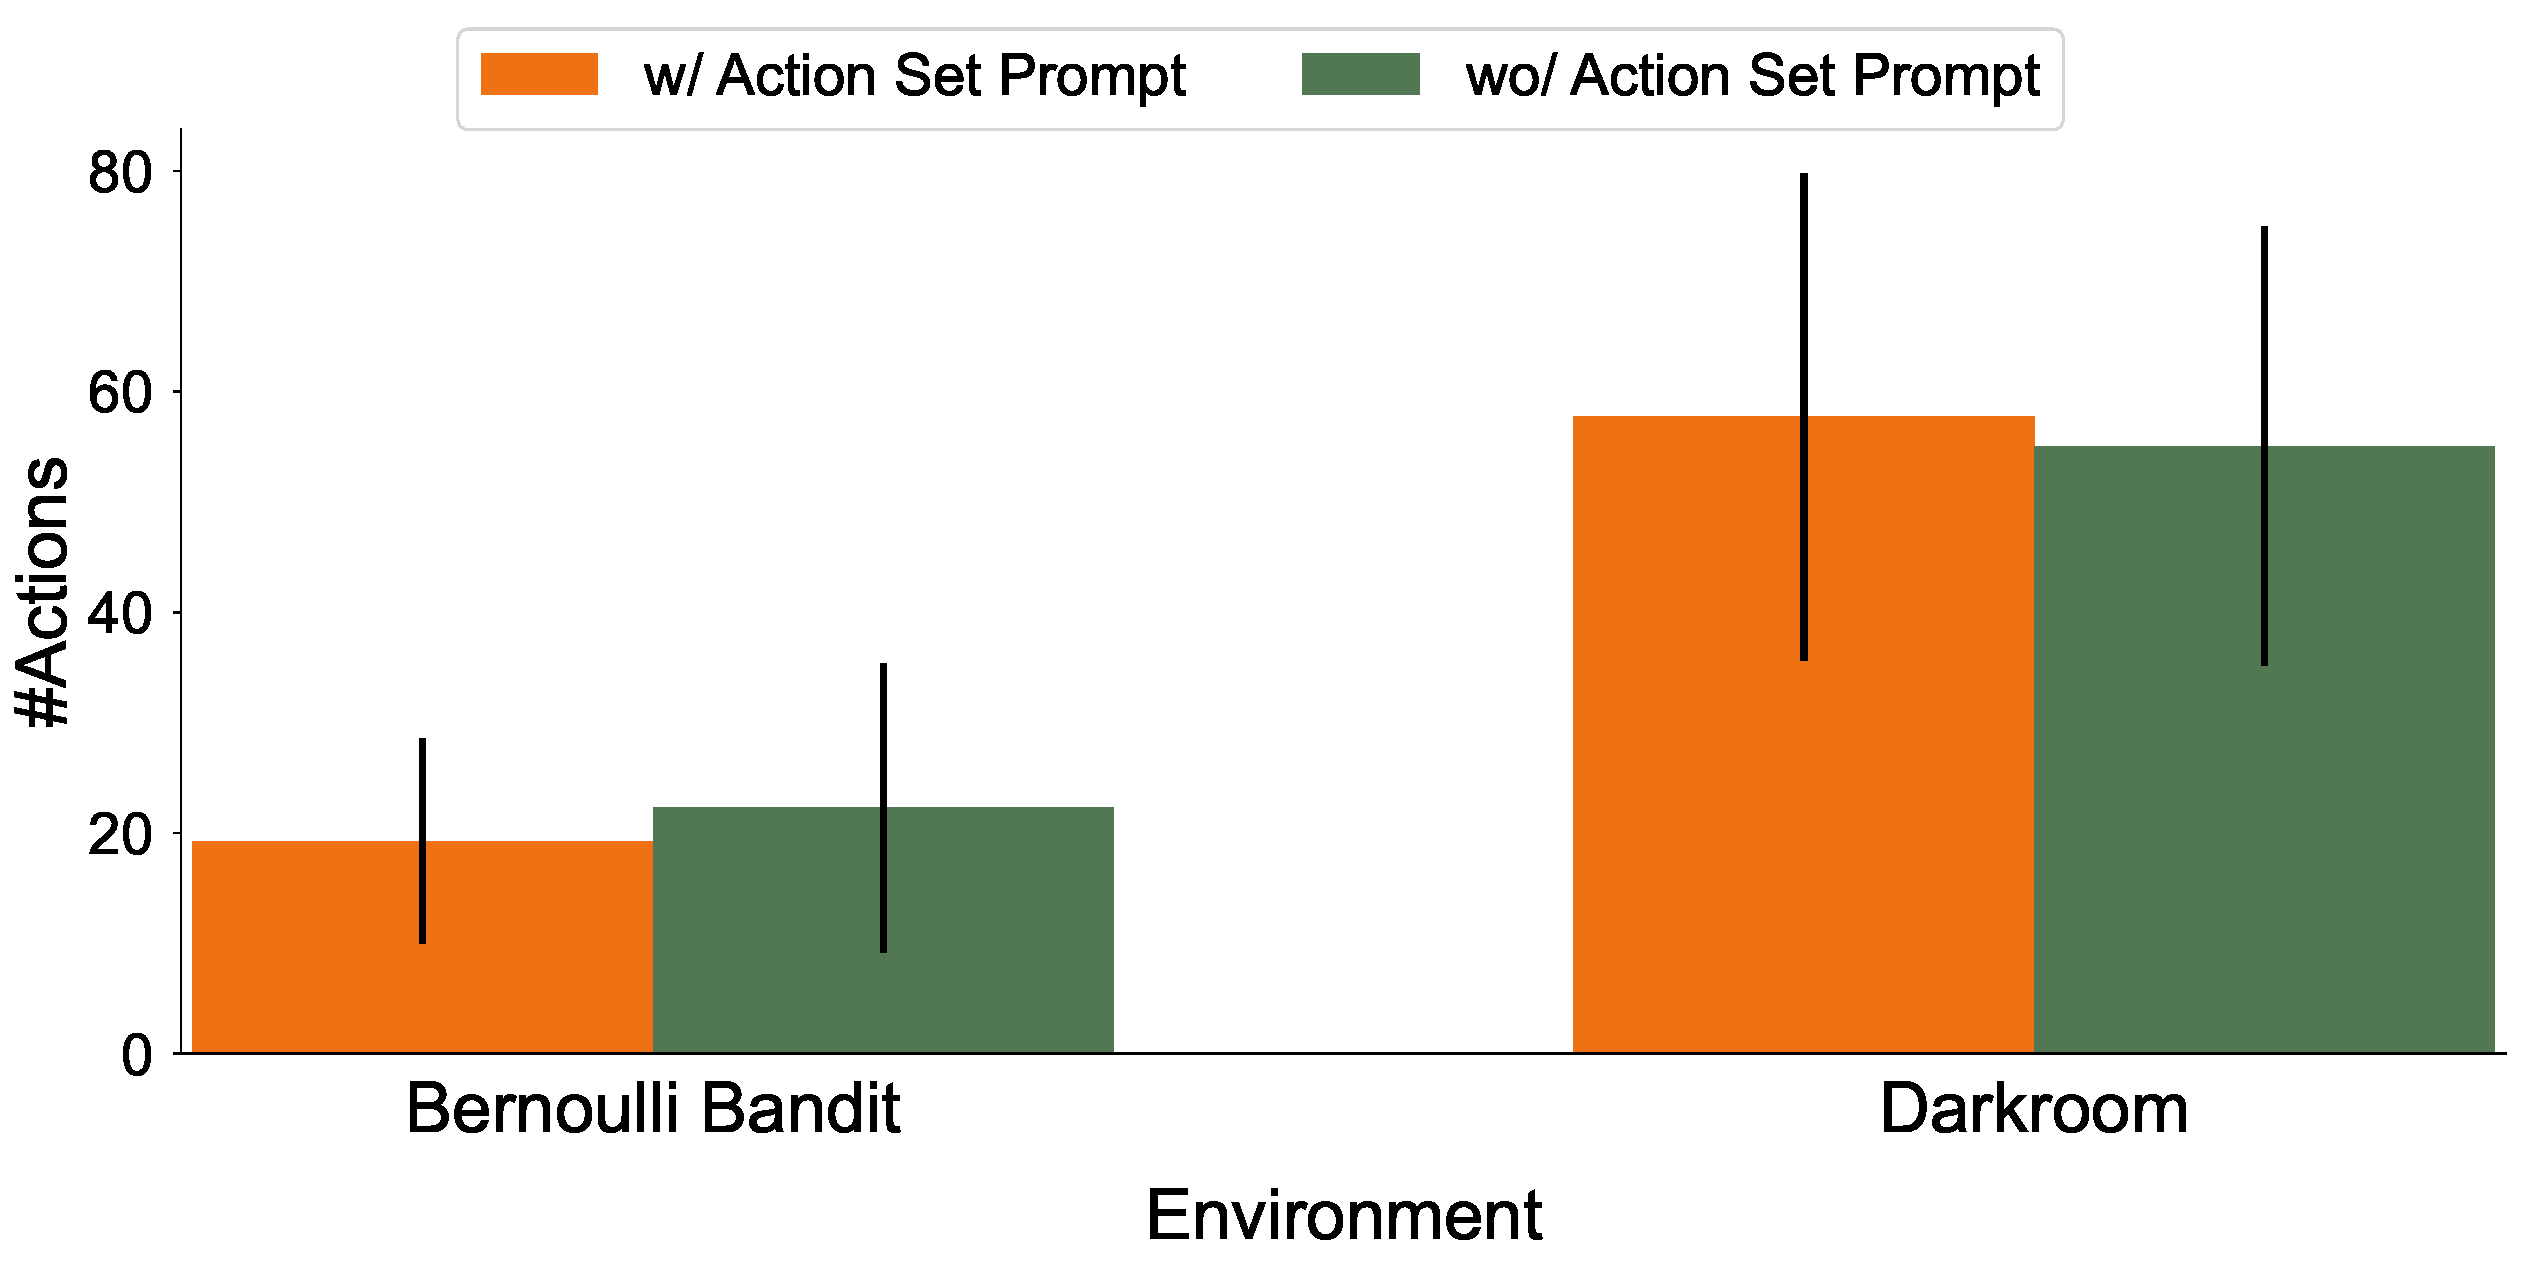
\includegraphics[width=0.85\columnwidth]{images/means_act_pool_ablation_num_acts.pdf}
%         \caption{}
%         \label{fig:means_act_pool_ablation_num_acts}
%     \end{subfigure}
%     ~
%     \begin{subfigure}{\columnwidth}
%         \centering
%         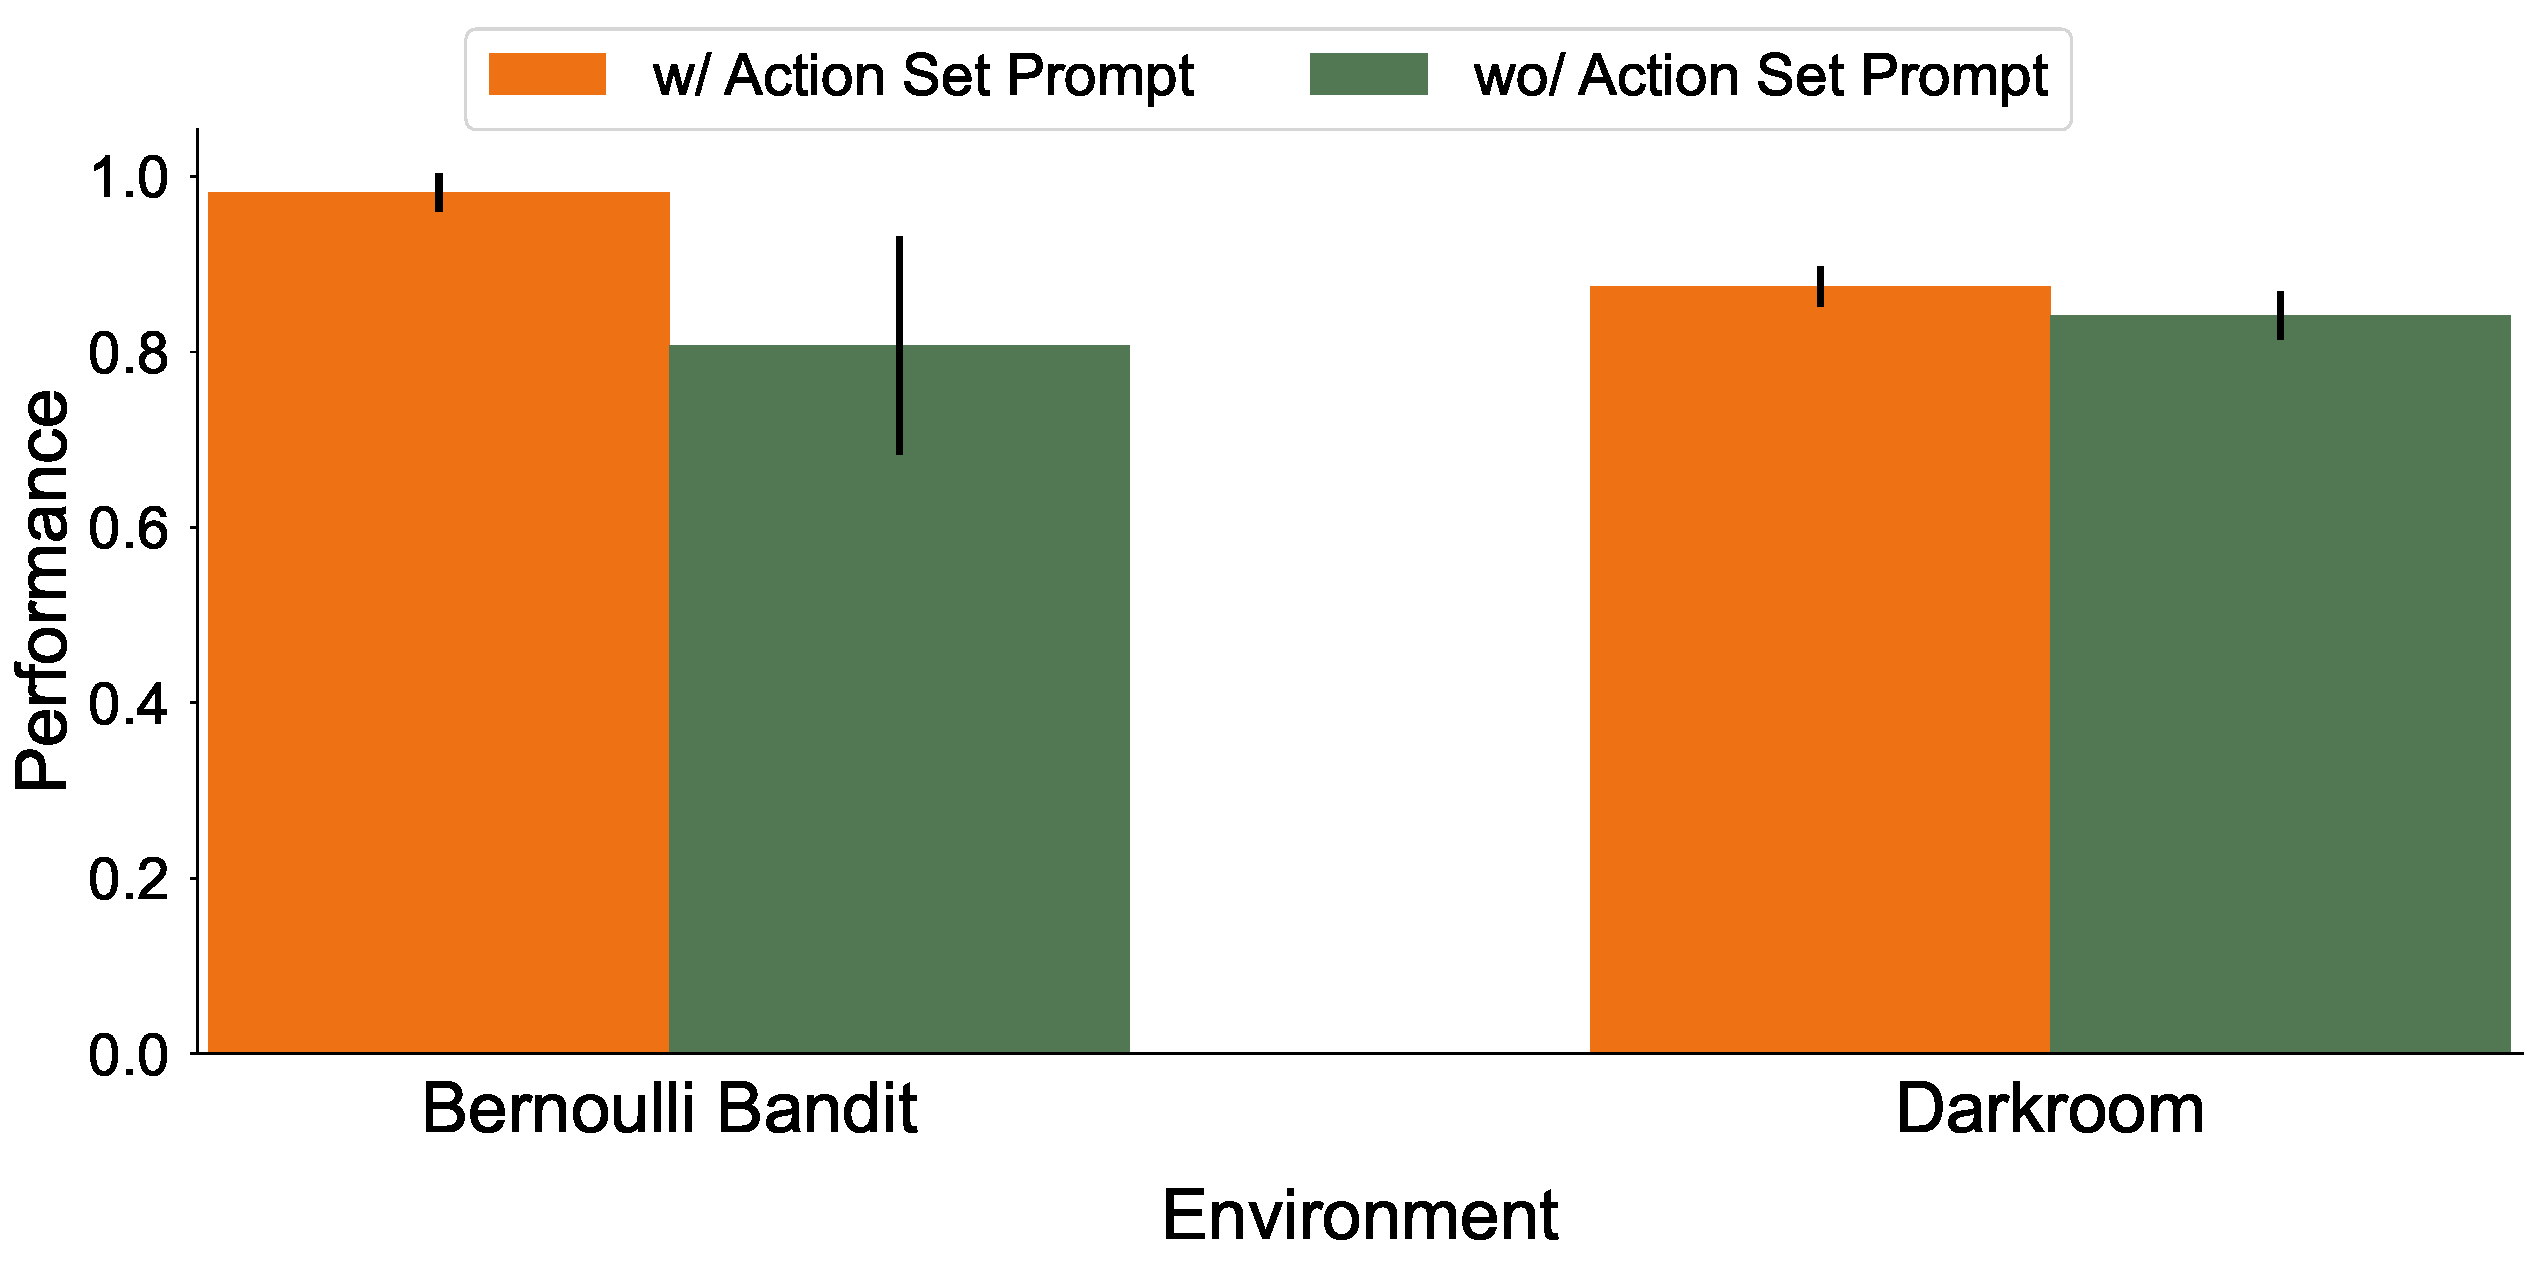
\includegraphics[width=0.85\columnwidth]{images/means_act_pool_ablation.pdf}
%         \caption{}
%         \label{fig:means_act_pool_ablation}
%     \end{subfigure}
%     \vfill
%     \begin{subfigure}{\textwidth}
%         \centering
%         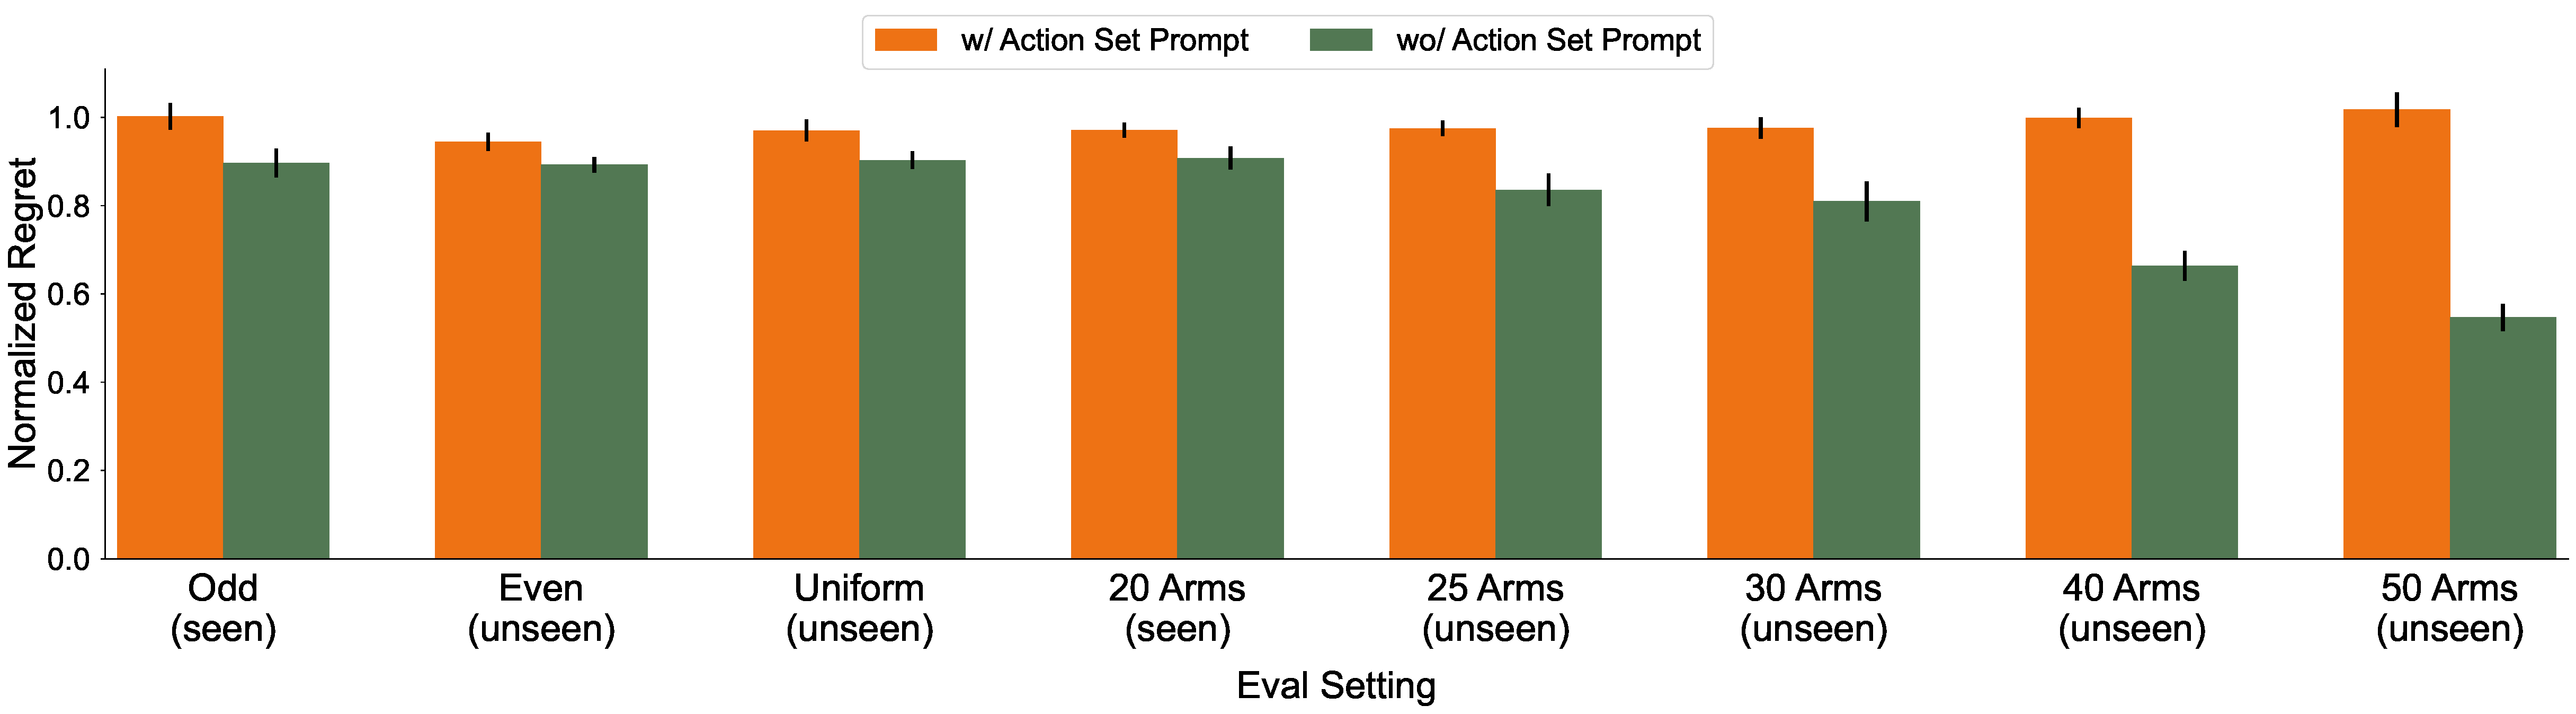
\includegraphics[width=0.95\textwidth]{images/bandit_act_pool_ablation.pdf}
%         \caption{}
%         \label{fig:bandit_act_pool_ablation}
%     \end{subfigure}
%     \caption{\textbf{Impact of Action Set Prompt Ablation:} (a) The inclusion or exclusion of the prompt, which lists all possible action embeddings, does not substantially affect the number of distinct actions explored by the agents. This plot shows an averaged number of actions values across all action sets. (b) The exclusion of the prompt significantly impacts performance in environments like the Bernoulli Bandit, while the effect is less prominent in the Darkroom environment. This plot shows average performance values across all action sets. \textit{Performance} on the y-axis represents the normalized regret on the Bernoulli Bandit environment, and the success rate on Darkroom. (c) The exclusion of the prompt has an impact on performance that becomes increasingly significant with the growth of the action space. The trend suggests that, as the number of potential actions rises, the ability to strategically sample actions based on the action set prompt becomes increasingly vital for model efficacy.}
%     \label{fig:act_set_prompt_ablation}
%     \vskip -0.2in
% \end{figure*}

\textbf{Results and Discussion:} \Cref{fig:gridworld_bars} illustrates the generalization abilities of both AD and Headless-AD. First, note that both models maintain their performance when transitioning to novel tasks, thus fulfilling their purpose as ICL-RL models. However, this environment was mainly designed to challenge the models' generalization abilities on novel action spaces. Following the scope of the action space novelty we set earlier, we studied the models' ability to address changed action semantics and variable action set sizes. 

While AD achieves high performance on the train action set, its limitations become evident when the action space is changed. The first limitation is AD's action set size constraint. The linear layer at the end of its network fixes the size of the output dimension, something that cannot be modified once the model is trained. Increasing the amount of options, as was done in the \textit{Test Actions} and \textit{All Actions} sets, requires reinitializing the output dimension and thus retraining the model, which demands additional time and resources. In contrast, once trained, Headless-AD easily adapts to changes in the action set size without losing performance. 

\begin{table*}[!t]%htbp
\centering
\caption{\textbf{Ablations:} Table compares the performance of Headless-AD with its ablated versions. Columns 'Bandit' and 'Darkroom' show the performance averaged along all action sets. Bernoulli Bandit performance is normalized, where $0$ denotes a random agent and $1$ denotes the Thompson Sampling algorithm. Columns 'Bandit. Arms Used' and 'Darkroom. Arms Used' show the amount of actions tried by the model during evaluation, also averaged along all the action sets. Columns 'Bandit. \textit{N} Arms' show the performance of models on the Bernoulli Bandit environment for each respective number of arms during evaluation without averaging. The results are aggregated over $5$ random seeds. As the table shows, changing each component of Headless-AD's architecture greatly damages the model's ability either to utilize the action set effectively or to perform well.}
\label{table:ablations}
\resizebox{\textwidth}{!}{%

\pgfplotstabletypeset[
    font=\scriptsize,
    % style to set multiple columns with the same style
    % https://tex.stackexchange.com/a/272543/7561
    my multistyler/.style 2 args={
        @my multistyler/.style={columns/##1/.append style={#2}},
        @my multistyler/.list={#1}
    },
    create on use/row_names/.style={
        create col/set list={
            Headless-AD,
            Prompt Ablation,
            Loss Ablation,
            Embed Ablation
            },
    },
    columns/row_names/.style={string type},
    every head row/.style={before row=\toprule, after row=\midrule},
    every last row/.style={after row=\bottomrule},
    col sep=comma,
    columns={row_names,Bandit,Bandit. Arms Used,Darkroom,Darkroom. Acts Used,Bandit. 20 Arms,Bandit. 30 Arms,Bandit. 40 Arms,Bandit. 50 Arms},
    my multistyler={row_names, Bandit,Bandit. Arms Used,Darkroom,Darkroom. Acts Used,Bandit. 20 Arms,Bandit. 30 Arms,Bandit. 40 Arms,Bandit. 50 Arms}{string type},
    columns/row_names/.append style={column name=Setting, column type={l}},
]{tables/ablations.csv}
}%end resizebox
\vspace{-10pt}
\end{table*}

The second limitation is AD's reliance on a stationary action space structure. Due to the classifier nature of AD's network, it learns to associate each output dimension with a specific action meaning. When action semantics change either due to a permutation of seen actions, as in \textit{Permuted Train Actions}, or due to a substitution of completely new actions, as in \textit{Sliced Test Actions}, AD's performance degrades. We checked whether this problem may be solved by biasing the training distribution to have a structure resembling the one during testing. We trained AD on permuted action sets while leaving the data and the model architecture the same. However, as one can see in \Cref{fig:bad_ad}, this training procedure resulted only in a slightly decreased performance of AD in the \textit{Permuted Train} setting. An additional graph depicting the performance on each of the (action set, goal type) pairs can be found in \Cref{appendix:ad_perm}. Meanwhile, \textit{Permuted Train Actions} does not pose a challenge for Headless-AD as, by design, it is invariant to specific action order. Most importantly, Headless-AD maintains its performance even when completely new actions are introduced, despite having never seen them in training. We attribute this feature to our success in making the model infer action meaning from the context.


